\begin{figure}[htbp]
  \centering
    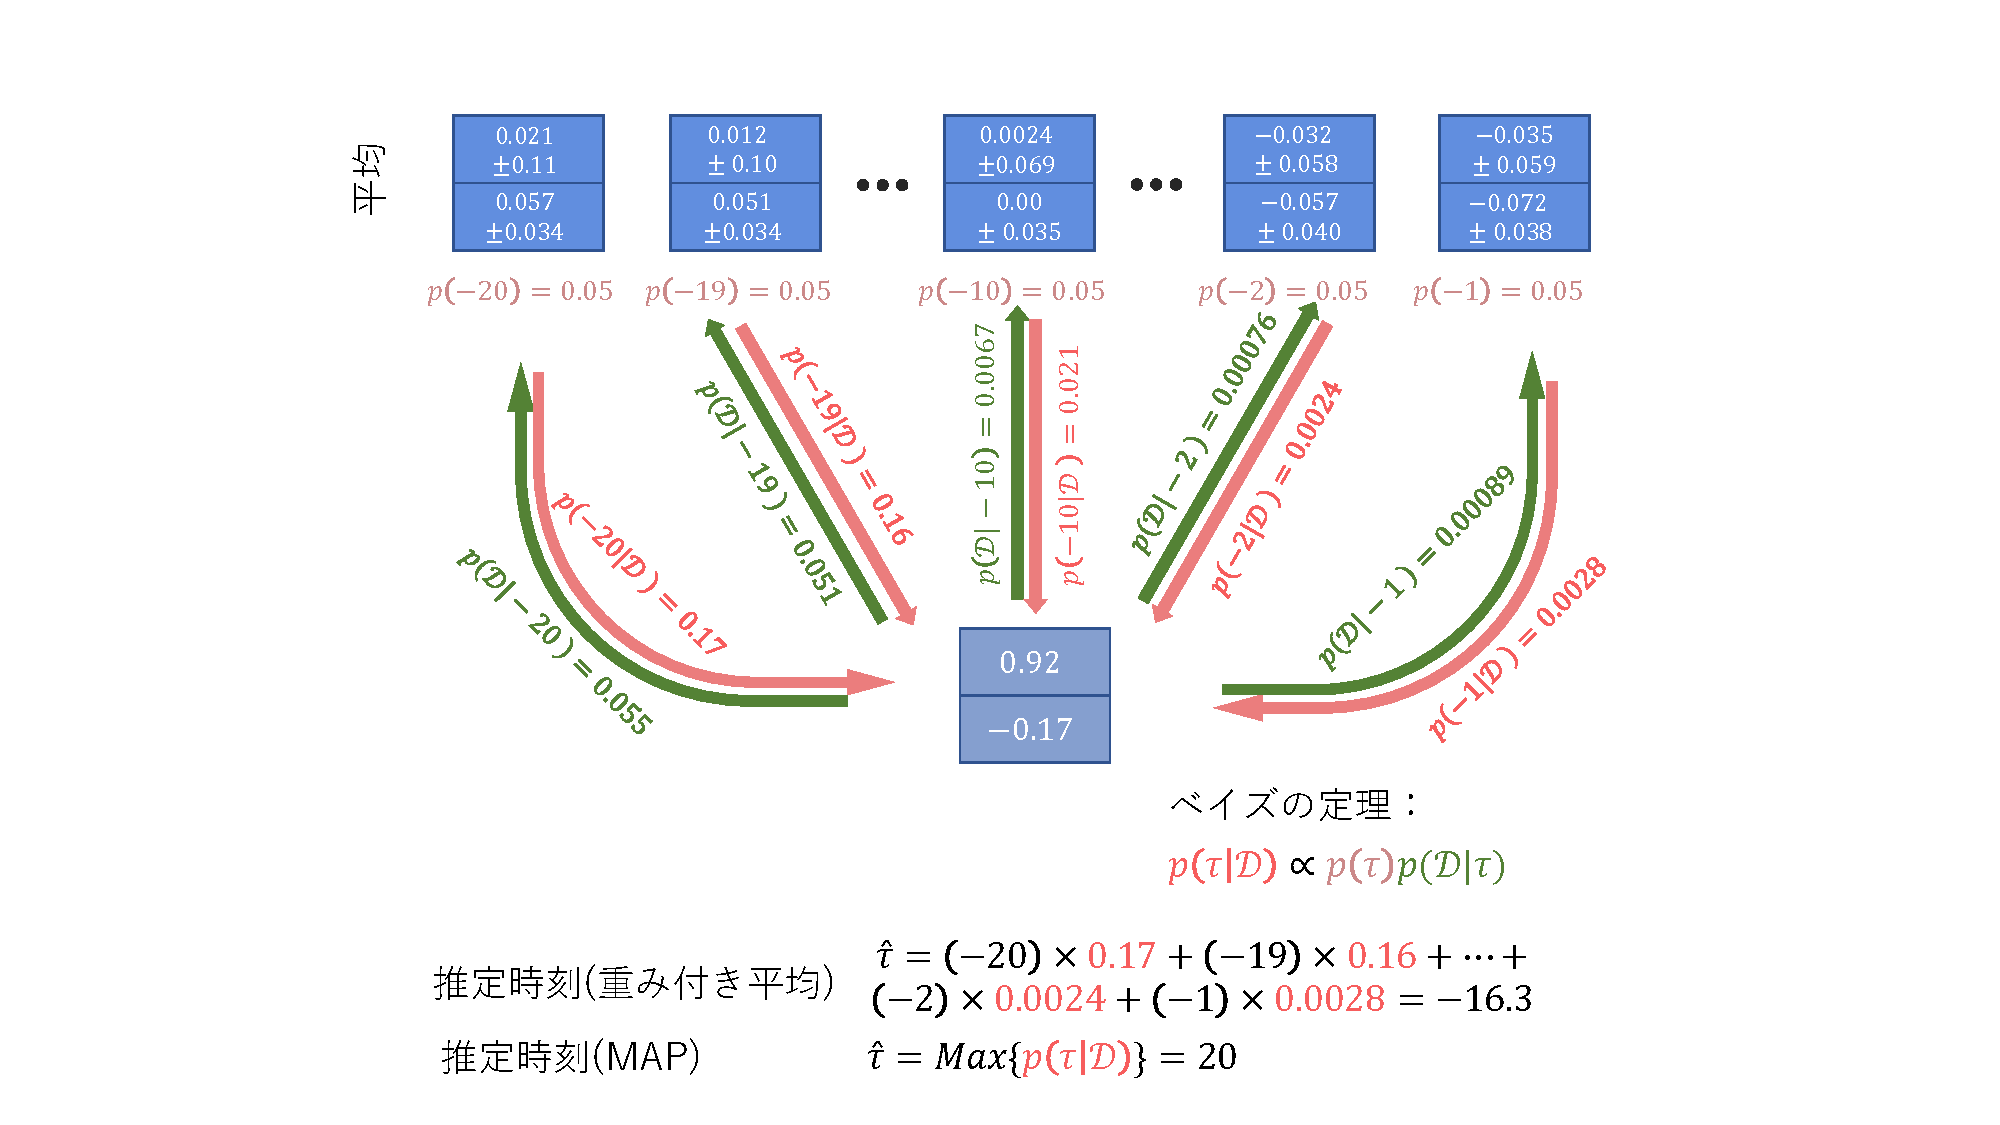
\includegraphics[width=11cm,keepaspectratio]{fig/update_flow.pdf}
  \caption{各時刻に属する正規分布から,現在の観測の尤度を求め,ベイズの定理により観測が得られたあとの分布を計算する様子を図示したもの.オレンジは事前分布,緑が尤度で,赤が事後分布を表している.また,図示した特徴量での例として,重み付き平均,MAPによる推定結果が幾つになるのかを示した.}
  \label{fig:update_flow}
  % figとfigure統一したかった
\end{figure}
